\documentclass[a4paper]{article}

\usepackage{ngerman}
\usepackage{graphicx}
\usepackage{hyperref}

\begin{document}


\section{Datenmodell}
Das vorliegende Dokument erklärt das verwendete Datenmodell. Sämtliche für die App nötige Daten sind im Source Ordner im Unterordner Data in der Datei med\_data.json 
hinterlegt. \href{https://github.com/pigutsche/dosi_calc/blob/main/src/dosi_calc/app/data/med_data.json}{hier einsehbar} Zum besseren Verständnis dieser recht komplexen json-Datei können die folgenden Diagramme und die dazugehörigen Erklärungen genutzt werden.


    \begin{figure}[h]
        \centering
        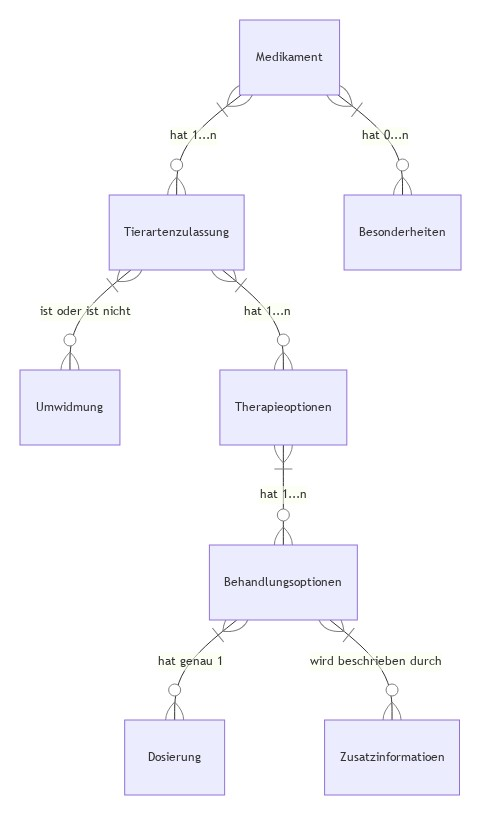
\includegraphics[width=0.7\textwidth]{er_diagramm}
        \caption{ER Diagramm der in der App verwendeten Daten}
    \end{figure}

Abbildung 1 zeigt das Entity-Relationship-Modell der Medikamente. Der Tierarzt wählt ein Medikament, welches dann für 1 bis n Tiere zugelassen wurde. Jedes Medikament 
kann dabei keine oder mehrere Zusatzeigenschaften (z.B. Reserveantibiotika, Sperrzeit, nicht für Lebensmittel) haben. Eine Zulassung zu einer Tierart kann eine Umwidmung sein.
Jede Zulassung zu einer Tierart erlaubt 1 bis n Therapieoptionen. Und jede der Therapieoptionen hat 1 bis n Behandlungsmöglichkeiten deren genaue Eigenschaften in den Zusatzinformationen
hinterlegt sind.

    \begin{figure}[h]
        \centering
        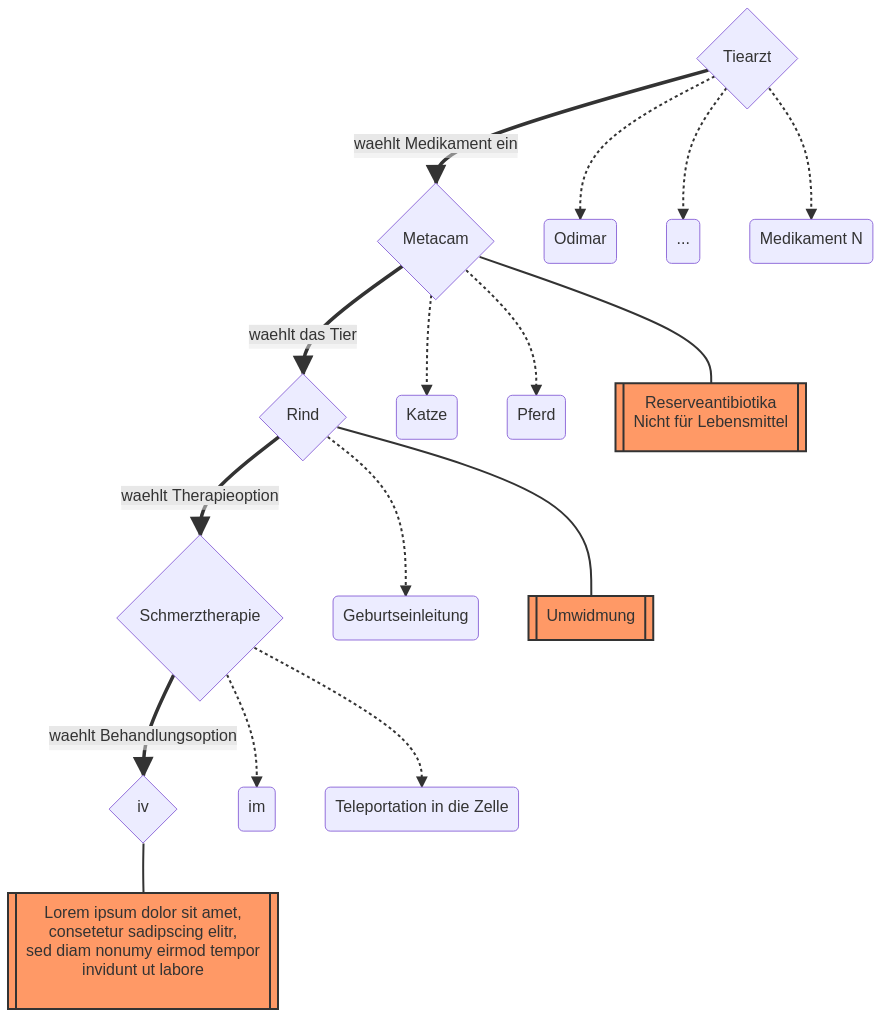
\includegraphics[width=0.7\textwidth]{flow_chart.png}
        \caption{Beispiel Ablaufdiagramm }
    \end{figure}

Der in Abbildung 2 dargestellte Flowchart zeigt dabei am Beispiel eines genommenen Weges die Auswahlmöglichkeiten des Anwenders. Dabei symbolisiert eine Raute mit dicken Pfeil 
den genommenen Weg und ein gepunkteter Pfeil die anderen möglichen Optionen. Die orangenen Kästen stellen die zu der Verzweigung gehörenden Eigenschaften dar. \\ \\

Aus den dargestellten Diagrammen und damit verbundenen Bedingungen an das Datenmodell wurde die Struktur der med\_data.json Datei erstellt. \\

Da zum Zeitpunkt des Projektabschlusses noch keine hinreichend große Anzahl an realen Daten Vorlag, verwenden wir zur Demonstration der App von uns erstellte Dummydaten.

    


\end{document}